Besides the lexical model, we also use an acoustic model to predict the punctuation.
The acoustic model is based on prosodic features, such as pauses and the pitch level.
In the following the training and evaluation of the acoustic model is shown in detail.

\subsection{Training instance generation}

Many researches are using pauses, the pitch level of the word, and its energy level for prediction punctuation.
Thus, we decided to also use this kind of features.

The pitch level encodes the volume of the speaker, whereas the energy level describes the amount of power the speaker is using in his voice.
To obtain those values from the \texttt{.sph} files, we first have to convert those files into \texttt{.wav} files.
We therefore use the library \emph{SoX}.
Having the \texttt{.wav} files, we can extract the pitch and energy level from them using different libraries.
For generating the pitch level the library \emph{aubio}\footnote\url{http://aubio.org/} is used.
The output is a file containing two columns: The first columns is the second in the talk and the second column is the pitch level of that second.
The library \emph{Yaafe}\footnote\url{yaafe.sourceforge.net/} is used for extracting the energy levels from the \texttt{.wav} files.
The output from \emph{Yaafe} is a file containing one column with energy values.
One line in the output file represents the energy level in \texttt{1/samplerate} intervals. \\

Together with the \texttt{.ctm} files, we can now create the training instances.
The process of generating the training instances is shown in Figure~\ref{fig:overview_acoustic}.


\begin{figure}[ht]
    \centering
    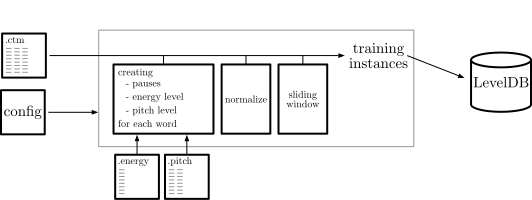
\includegraphics[width=\textwidth]{img/overview_accoustic.pdf}
    \caption{Creating the training instance for the acoustic model. The pause feature is extracted from the \texttt{.ctm} files, the pitch level feature from the \texttt{.pitch} files and the energy level feature from the \texttt{.energy} file. All features are normalized to a mean 0 and a variance of 1. Like in the lexical model, a sliding window is used to create the final training instances.}
    \label{fig:overview_acoustic}
\end{figure}



\subsection{Neural Network}

\subsection{Evaluation}

%\begin{figure}[ht]
%    \centering
%    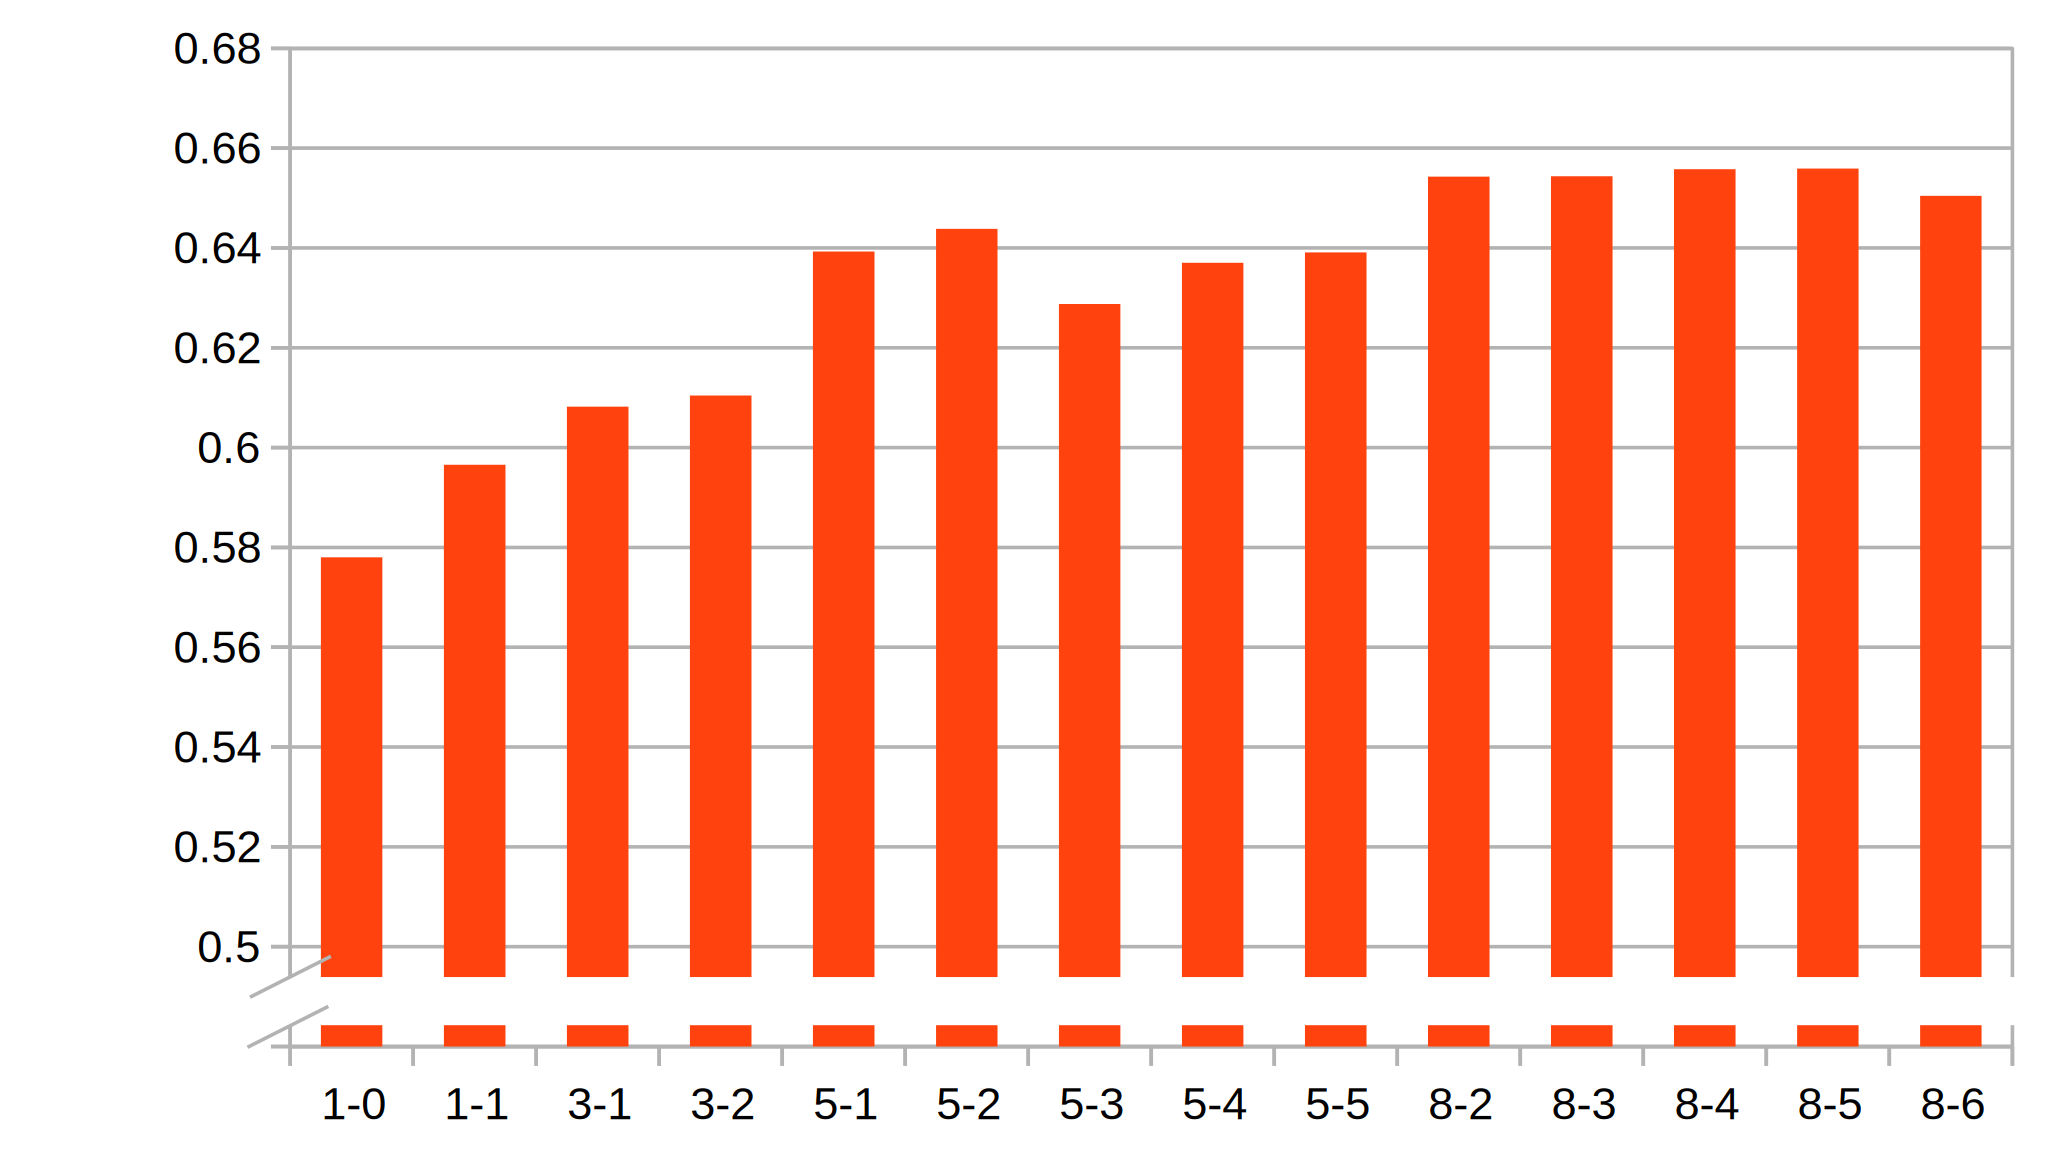
\includegraphics[width=0.5\textwidth]{img/audio_parameter_eval.png}
%    \caption{}
%    \label{audio_eval}
%\end{figure}